
%@author Brandon Roberts, Nate Olderman, Billy Rathje, DJ Maguddayao, Kyle Dybdal
%@date 9/23/13

\documentclass[12pt]{article}
\usepackage{graphicx}
\usepackage{hyperref}

\begin{document}

%-------------------------------------------------------------------------------------------------------------
% TITLE PAGE
%-------------------------------------------------------------------------------------------------------------

\begin{titlepage}
        \vspace*{\fill} %leave out given verticle space in a document
        \begin{center}
                {\Huge Story Creator Final Report}\\ [0.5cm]        
                
                %make title huge and have .5cm space in between
                {\Large Brandon Roberts, Nate Olderman, Billy Rathje, DJ Maguddayao, Kyle Dybdal}\\[0.4cm]
                \today %put the date that the data is compiled
        \end{center}
        \vspace*{\fill}
\end{titlepage}

%-------------------------------------------------------------------------------------------------------------
% PROJECT SUMMARY
%-------------------------------------------------------------------------------------------------------------
\section{Project Summary}
Edith is an online program that allows the user to create objects and program animations to move them. This allows the user to gain an understanding between how objects interact with functions in programming. The Story Creator module combines the Sharing Framework, Object Creator, Visual Editor and Animation modules in order to create a holistic view of Edith in a dynamic webpage. \\

The story creator (user) will be directed to a login page that will prompt them for their username and password. If they do not have an account they may create one in the link that says "Create Account."  In the case that they have already have an account they will be directed to the main Edith page where they will be able to create a "story." To do this they can click on the button that says "Make Object." This will redirect them to a new page that allows them to create new objects with the ability to free draw, create circles, and create squares. After the user finishes creating objects they will export the object and enter the name that they wish to use for the object. The user can then navigate back to the main page and click the load button. After entering the name of the object that was exported, the object that they created will appear on the bottom canvas. Then the user may double click on objects (this adds the objects to the canvas and allows the user to animate them). The user can also single click objects. This makes the objects glow and means that they are currently selected for programming in the visual editor and for animating on the canvas. The Story Creator can then give the objects animations by manipulating the functions in the Visual Editor canvas. The Visual Editor canvas has several coding blocks which correspond to built-in methods for animation (e.g. jump, rotate), logic choices like \texttt{if} and \texttt{else}, and program flow functionality like functions. By doing this, students will be able to learn how relationships among objects work in object-oriented programming. \\

The Story Creator Module designed the Edith main page, login page, and sign up page. A large portion of time spent by the Story Creator module went into the creation of the three major canvas' on the page that were for the Animation, Object, and Visual Editor Modules.  These were created and formatted correctly for what each team needed. The Visual Editor and Object Creator module implement a Kinetic canvas while the Animation team utilize an OCanvas. The canvas for Objects was directly implemented in order for objects saved to the Sharing Framework to be displayed in the canvas. The Story Creator module also added the functionality of clicking on the objects to make them glow and put them into an array for the Visual Editor module to implement.   


%-------------------------------------------------------------------------------------------------------------
% DEVELOPMENT PROCEDURES
%-------------------------------------------------------------------------------------------------------------
\section{Development Procedures}
In order to complete Edith the Story Creator module followed the iterative, extreme programming, and the Boehm spiral model.  We initially used the Boehm spiral model by determining our objectives, identifying risks, testing, and planning our next cycle.  We found quickly that this was not the most applicable model because of the amount of changing requirements, which forced us to throw away old code.  In order to use the Boehm spiral model we considered what it would take to complete our module and have all of the modules working together.  We also attempted to minimize risk by determining how much we needed to integrate the teams early on.  The Boehm spiral model helped to determine how much detail needed to be implemented in order to group modules together.  It transformed into an iterative model because we discovered that we had to repeatedly redo our entire module due to changing requirements and specifications from other groups and the project as a whole.  
\begin{itemize}


\item We began implementing the functionality of receiving JSON objects, adding a time to them, and passing them on to other groups. 

\item We also added the functionality to set a time to wait for a function (this was later transferred to Animation) inside the code which allowed the user to specify how long a function should wait before executing. 

\item Later our requirements changed completely and we began creating the base webpage view for the entire project. 

\item Then, we worked on incorporating the Visual Editor canvas into the main page, setup a main canvas, creating dummy buttons for different functionality, and the canvas for viewing objects. 

\item From there we worked on design for the login page, main page, and the registration page. 

\item We then worked on getting the AJAX calls up and working with the Sharing Framework.   

\item We assisted the Object Creator and Sharing Framework modules with saving and loading from the database as well as setting up the save and load for the entire project. 

\item We worked on connecting the various elements from the main page with the groups that they corresponded to.  This included loading data from the database and displaying it on the object canvas.  \\

\end{itemize}

Because of how collaborative our process model was, we also made frequent use of pair programming. We did the majority of programming together as a group, and while individuals often wrote sections of code, we would each look at each others code either as it was being written or immediately after. This helped both to catch bugs and to ensure that everybody understood the entire code base. \\

Our process was inefficient because we created working software that was never used or even thrown away.  The requirements for the Story Creator module changed frequently because the modules that were supported by Story Creator changed how they implemented certain aspects of their project.  The changes that were needed by the other modules would no longer function with the previous code that the Story Creator module implemented and ended up being thrown out.  We mostly implemented console log testing and used JSHint.  The JSHint was used later in our process when implementing the glow function as well as adding images to the object canvas.  Our program works because the main page displays all canvases as well as allowing the other modules to function correctly on them.  The object panel at the bottom of the screen also displays the objects correctly.  Console log testing was effective for showing us how the page interprets the information that we were displaying.  JSHint was effective at showing us syntax errors in our code.  At times console log testing was ineffective at pointing out why our code was not functioning.  We logged information gathered from the user that was then placed in the \texttt{addSprite} function to set the original location of the sprite.  The sprite would not display even though our console logs determined that the number received from the user were correct.  We determined on our own that the input from the user was not turned into an integer but rather a String that would not work correctly in the \texttt{addSprite} function.  We originally console logged the variables input by the user which displayed the correct number.  We then used hard coded values to make sure that the \texttt{addSprite} function worked correctly with integers.  We attempted to code in hard coded numbers for the variables used in the function and log those (they displayed correctly as well).  After this step we worked to find out if there was an issue with the variables changing when put them into the function (console log before and after we used the function).  We then just came up with the idea that the parameters needed for the function were not correct.  We fixed the issue by turning the variables used in the function into integers right before we called it.  \\



We did both formal testing and informal testing throughout the process of putting together the project. Formal testing involved static analysis and unit tests designed by another group. These helped resolve bugs, but our project specifications changed drastically after testing, so we employed frequent informal testing as an adjunct. This formal testing involved printing and manually interrogating the state of all data structures we produced. Because story creator passes data to multiple teams, ensuring that data structures such as the array that holds highlighted objects are working correctly is imperative. We typically investigated the state of these data structures with multiple conditions (often looking closely at boundary conditions like zero items, several items, one items) to ensure that they worked correctly. However, since the majority of our work involved designing the central website, the vast majority of testing involved simply viewing the website to make sure that it displayed properly. There is no direct way to test, for example, whether object images fail to load except through manual investigation. We frequently examined our interface carefully and by hand to ensure it displayed well, looked to the browser debug console for hidden (or sometimes clear) errors, and tested the website in several browsers and configurations (relatively simple because we all use different browser configurations) to ensure that the implementation was robust. \\

\subsubsection{Responsibilities}

For the initial product that was later scrapped, Nate was responsible for designing some of the dummy files that were made to represent the other modules. He was also responsible for connecting these files to our code so we can access the information and test our module. For the final product, Nate was responsible for how the various canvases were drawn on the Edith main page as well as their relative sizes to the window. He implemented the canvas' resizing capability for whenever the user resizes the webpage. He also worked on various bug fixes, cleanup of antiquated code, and implementation of many small functionalities (e.g. button method calls). He helped implement the functionality of getting objects from the object creation page into the object canvas below the main canvas. He then wrote and implemented the tutorial on the webpage. \\

Originally Brandon was responsible for retrieving data from JSON objects and creating a new JSON object with the user specified time of delay for a generic function.  Then Brandon was responsible for helping the Object Creator module and Sharing Framework gain access to the database with JavaScript.  This included writing load and save functions for the main page that sent and retrieved data.  Brandon was also in charge of porting the Visual Editor code and the Object Creator code so that it would function on the main page.  Finally Brandon was in charge of loading data from the database in order to draw objects on the object canvas that were clickable.  \\

Kyle was responsible for much of the design of the website. This process started with making a website mockup, and then designing a logo and color scheme. Lots of work was done with HTML and CSS, putting together the general layout of the page. The goal of the design was to be minimalist and out of the way, keeping as clean of a workspace as possible. He also created the login and registration page. \\

Before changing requirements, the Story Creation team worked on adding timing to the Visual Editor's code. In the initial demo, Billy contributed to functionality for adding images to the page/canvas, designing the JSON representation of objects and time, and contributed to developing the page layout. Billy also planned and added some of the initial frameworks, like jQuery, and refactored some of the initial code. Billy was responsible for designing, styling, and implementing the object browser panel. He wrote the code for displaying objects in a grid, adding objects individually and from an array, and for sizing/positioning objects. He also worked on CSS styling for the object panel. He implemented a Kinetic JS canvas so that the panel could display objects. He also implemented the "glow" or highlighting functionality which highlights objects and places highlighted objects in an array that the Visual Editor accesses through an accessor method. He worked on some of the data retrieval code (particularly for displaying objects designed in the Object Creation panel) as well as server setup/testing. He also contributed to some of the page layout/design. \\

Before, DJ worked on small fixes to the program itself.  Not much has actually changed in the later parts of the project.  Rather than working on actual code, he had looked over other member's code on the main page during creation and adding small things such as the scroll ability on the visual editor canvas.


%-------------------------------------------------------------------------------------------------------------
% REQUIREMENTS EVALUATION
%-------------------------------------------------------------------------------------------------------------
\section{Requirements Evaluation}
\subsection{Functional Requirements}
\begin{itemize}
\item "Navigate Story Files" - The storyteller will have the ability to start a new story file, save a story, and close a story.\

\textit{This is a valuable requirement because it allows the entire story to be able to function, but it is possible that it could have been broken into multiple components like "new story," "save a story," and "close a story."  This requirement enables the storyteller to begin their story and come back to it later.  We were not able to complete the "close a story" option.  The current story is set as a project and is loaded from the sharing framework.  The option to close a story was not completely necessary in the end because the user still has the option to make a new story and begin it. If we had broken this into three components, we could have considered the feasability or necessity of each part in isolation.}

\item "Start a new story file" - The storyteller will select an option to create a new story.\

\textit{The option to start a new story is not available.  This requirement was not defined well because the "starting a new story file" does not specify if the old one is saved or if there is an option to use pieces from the previous story.}

\item "Save a story" - The storyteller selects the option to save the story.  A representation of the story and its objects, scripts, and settings is sent to the Sharing Framework.\

\textit{This was a very useful requirement because it allows a previous story to be loaded onto the screen after being saved, which is a helpful feature for users who want to continue projects.  It was very effective because it was a great way for AJAX to be used in order to retrieve necessary information from the database.}

\item "Close a story" -  The user selects an option to close the story.  The story is removed from the story editor and animations, scripts, and objects associated with the story are cleared from their respective editors.\

\textit{The ability to close a story is not an option.  This requirement seemed unnecessary because the storyteller can load a separate story without closing an old one.  At the end of the process closing a story did not seem very important.}

\item "Create an object" - Storyteller will go to the Object Creator screen. Storyteller will select an option to create an object.  Storyteller will use the mouse to drag the object. Storyteller will choose where to place the object. Storyteller will drop the object in that place.\

\textit{ The ability to create objects and add them to the scene is fundamental to making Edith a functioning visual programming system. As a result, this requirement was very important, although it would have been helpful to split it into two requirements, one for making objects and one for adding objects, since these both ended up being complicated functions designed by different teams. The final implementation worked such that an object was created in the object creation window designed by the Object team. When finished, this was uploaded to the server and added to the object browser through an AJAX call to the server from the main page designed by the Story Creation team. Adding objects to the canvas is done programmatically within the code made by the Visual Editor team. In the visual editor panel is a function \texttt{addObject()} which adds an object to the animation window. As a result, there was no need to use a drag and drop interface to move objects to the canvas. The Visual Editing team decided on this option in order to allow objects to be added as part of an animation; with the drag-and-drop approach, objects would have had to be present at the start of the animation to appear in the story.}

\item "Remove an object" - selects an option to delete objects. User selects the object to delete. The object disappears from the scene.\

\textit{This function is not present in the final implementation. It was originally intended to be used with the previous functional requirement so that if an object was dragged onto the animation canvas it could be removed from the canvas. Since objects are no longer dragged onto the canvas, there is no need for a remove feature. This functional requirement would have been useful had we kept the old implementation, but it is no longer necessary. If we had broken up the previous functional requirement into two functional requirements, we might have been able to decrease the ambiguity surrounding what it means to "remove" an object. We do not need a feature to remove objects from the animation canvas, but removing objects from the object browser might have been a nice feature. If we had decoupled the previous requirement into create an object and add an object to scene, we might have thought to have added functional requirements for remove object and remove object from scene. "Remove object" may have been a nice feature for the final implementation.}

\item "Move an object" - User selects an option to move objects. User drags the object from its original location to a new one. (This is not an animation)\ 

\textit{Since the ability to drag and drop objects (see last two requirements) is no longer part of the final implementation, there was no need to implement the "move an object" functional requirement. It would have been used to position objects using drag-and-drop on the animation canvas. Instead, this functionality is handled via parameters in the Visual Editor's \texttt{addObject()} function. This approach is similar, and is probably better for teaching users early on how to program using function parameters. The old requirement would have been useful, however, had we kept the drag-and-drop approach.}

\item "Develop or edit a script" - Storyteller interacts with the visual editor to develop a new script. Storyteller selects a specific action which is an individual script (All of the scripts interact in a main loop).\

\textit{The ability to develop or edit a script is central to the final version of Edith. Creating an animation centers around using the visual editor to develop scripts that animate objects as well as a main method that calls these scripts. This requirement was met. The Visual Editing team developed a visual programming interface for writing functions, loops, conditionals, and program logic, which can be combined together into scripts. The Visual Editor assigns scripts to objects that are highlighted in the object panel designed by the Story Creator team; if no object is highlighted, the script is not used for any particular object (like a global/scene wide function) or is part of the main method. The implementation of this requirement changed somewhat over time. Initially the Story Creation team was going to assign time values to functions made in the Visual Editor, but timing is so essential to visual editor functions and scripts that Visual Editor incorporated timing parameters into the Visual Editor interface.}

\item "Delete a script" - User interacts with the visual editor to delete a script.\ 

\textit{In the final version of Edith there is no ability to delete a full script since there is no interface displaying full scripts. However, this functional requirement can be achieved; a user could interact with the visual editor to delete all the code for a single object or for an entire story, then save the story to record the deletions.  Deleting a script is not a set functionality that the user can naturally do with one click.  Instead they must remove every piece of the script in order to fully delete it. There are options to delete functions and other program logic from the Visual Editor panel. This is done by dragging function/logic/programming blocks out of the right half of the panel. The functional requirement was useful because the functionality it proposes is present in the final version of Edith. However, it may have been better in retrospect to have used a finer level of granularity in describing the functionality and discussed deleting individual logic/object/functions.}

\item "Save an object or script" - The user wants to save an object or script for reuse. A representation of the object or script is saved.\

\textit{We were able to save objects for reuse by having JS functions "grab" the object exported by the Object Creator module. We did not implement saving of scripts individually; scripts must be produced on the fly for each new project. However, this appears to be something that would fall under Visual Editor's responsibilities rather than our own.}

\item "Animate an object" -  User selects a script from the visual editor. User drags or otherwise attaches the script to an object in the scene.\

\textit{This requirement changed over time due to changes in the interaction with and responsibilities of the Visual Editor module. Animation was achieved by having standard functions that apply to all objects that take the target object as a parameter. The Storyteller can highlight multiple objects for a function in the visual editor to act upon.}

\item "Play story" - Storyteller selects a "play scene" option. The story plays for the storyteller in the animation viewer at the beginning.\

\item "Share a story" - User selects a "publish story option." The story is converted to a representation that the sharing framework can read. The story representation is sent to the sharing framework so that it can share the scene.\

\textit{This was achieved through the use of AJAX communicating with the PHP on the server set up by the sharing team. The project is saved as a JSON object, which can then be loaded again.}

\end{itemize}


\subsection{Non-Functional Requirements}

\begin{itemize}

\item "Ease of Use" - The number of errors made by experienced users may differ significantly from those made by first-time or novice user. An experienced user should make no more than 3-5 errors per hour. While there is some complexity to the story editor, an experienced user should not have trouble knowing which options to choose to add objects or play the scene. \\

\textit{We never performed any studies to quantify the number of errors made when using Edith, although this could be future work for the project. Judging from anecdotal evidence, it appeared that the system was relatively easy to use (with some instruction from the various teams) during integration demos. Since most of the teams were using parts of Edith designed relatively recently, they could be considered "novice users." Their general ability to learn and use the system readily suggests that Edith is relatively simple for novices to learn. In the sense that this nonfunctional requirement is specific, it is a useful requirement, but in the sense that testing it involves procedures that we never did, it may have been too difficult a requirement to adhere to effectively.}

\end{itemize}
%-------------------------------------------------------------------------------------------------------------
% SYSTEM DESIGN AND ARCHITECTURE
%-------------------------------------------------------------------------------------------------------------
\section{System Design and Architecture}

\subsection{High-Level Architecture}
The story creator module of Edith is responsible for connecting the various other modules to each other and the user. This is mainly done through the design, layout, and functions of the webpages. The first page the user sees would be the login page. Here we designed a page for people who have already registered to type in their username and password. From there it gets passed to the sharing module which checks to see if they already have an account, and if their username and password is correct. The user can also choose to register by clicking on the register button. This loads the registration page, which allows the user to enter their information. This information is also passed to the sharing module. Once the user has logged in, they will be on the main page. \\

The main page connects the user to each of the modules. On the right side of the page is the visual editor canvas, this canvas is connected to the visual editor code so the user can interact with it and write code themselves. On the bottom left of the page is the object viewer canvas. This canvas allows the user to view the objects that they have loaded or created through the object creator module. Above this canvas is the main canvas, where the user can view the animations they have coded on the objects they selected. On the top part of the page are five buttons. One calls the animation module with the code they made in the visual editor module; this call allows objects to be animated on the main canvas. Another button calls the object creator module, which allows the user to make objects. The other three buttons call the sharing module that allows the user to save and load their project and display their projects. \\

The main page also connects the some of the modules together. The visual editor canvas interacts with the object viewer by allowing the user to select an object and add it to their code. This connects the visual editor and object modules. The main canvas connects the animation, visual editor, and object creator modules. The main canvas displays an object from object creator module, code is called on it through the visual editor module, and passed to animation module to make the object animate. 

\begin{figure}
    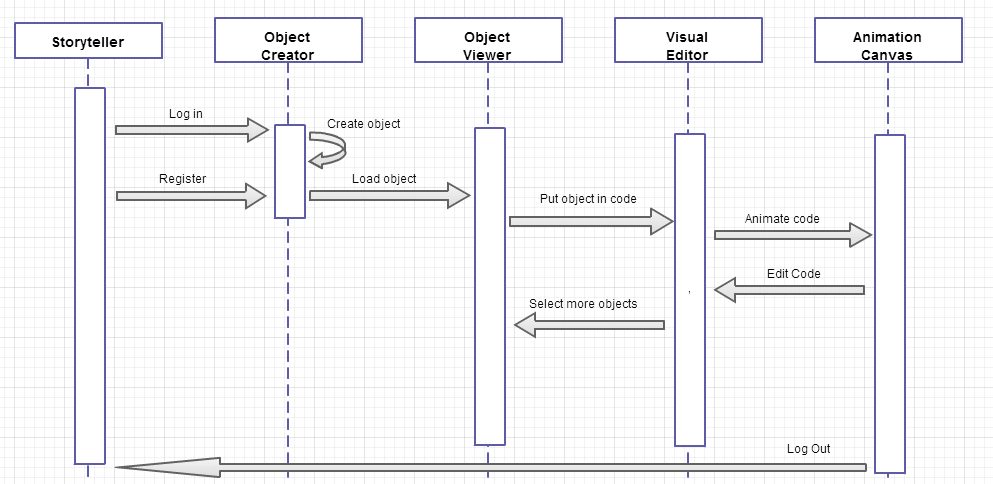
\includegraphics[scale=0.5]{HighLevelArchitechtureUML.png}
    \caption{A sequence diagram for the High Level Architecture of the main page}
    \label{Figure 1}
\end{figure}


\subsection{Low-Level Walkthrough}

Resizing code and server-interfacing code appears in a script on the main Story Creator webpage, \texttt{mainpage.html}. The object panel is relatively independent from the webpage so its code appears in a seperate file, \texttt{objectPanel.js}, which the webpage imports. There is also login code in the pages \texttt{index.html} and \texttt{registerpage.html}. This walthrough will first address the code in \texttt{mainpage.html}, then it will address the code in \texttt{objectPanel.js}, then it will address \texttt{index.html} and \texttt{registerpage.html}. \\

\subsubsection{index.html}
\texttt{Index.html} is our login page, and is connected to the main page and register page by the sharing team. The CSS implements a radial gradient in the background, and a centered logo and field for inputs. There is a wrapper around all the text and input fields to keep them all centered. Input fields are positioned relative to each other, and both they and the buttons change color upon hovering. The font Roboto Slab was imported, as it complements the font of the logo.\\

\subsubsection{mainpage.html}
\texttt{Mainpage.html} starts with a series of imports. The page imports the KineticJS canvas library, JQuery, JQuery UI, visual editor's canvas JavaScript code, visual editor's sortable JavaScript code (for sorting visual code blocks in the visual editor canvas), object creator's JavaScript code, and animation team's JavaScript code. \\

The CSS code sets up a linear gradient background. It positions the logo on the page absolutely and assigns positional properties (width/top/left). It also assigns positional properties for the animation, object, and visual editor container and gives them borders and background colors if appropriate (animation has no background color). The buttons and container div tags are also styled so that they are positioned properly on the page. Positioning for all containers is absolute, so that they are responsive to re-sizing. Slight drop shadows and rounded corners were added to cleanly separate the various windows. Some elements, like the gradient, change based on the browser being used. \\

Next, we set up the page's basic layout in HTML. We start by making div regions for the heading/logo, the main animation canvas, the object browser, and the visual editor canvas. We import the \texttt{objectPanel.js} script in this section as well. \\

The next part of the page is an embedded JavaScript. The script first handles page sizing by setting \texttt{height} and \texttt{width} variables for each canvas. There is a function that does this again each time the page is resized so that the canvases resize relative to the overall page size. Sizing is handled by setting canvases to various ratios of the window's current width or height, which is found with the JavaScript parameters \texttt{window.innerWidth} and \texttt{window.innerHeight}. \\

The next part of the script consists of three functions: \\

1) The function \texttt{popitupObjc(url)} creates a new window when given the url for a page. This is used to open the object creation page in a new window. Next is the variable declaration, \texttt{projectCode}, an array which stores the JSON representation of the currently open project (or an empty array if no project is open/if a project fails to open). \\
\indent 2) The function \texttt{loadProject()} makes an AJAX get request to Sharing Framework's file \texttt{load.php} to get the project JSON associated with an id. Upon a successful get request, the function obtains the variable \texttt{unstring}, a JSON representation of the project, which is parsed into an array using \texttt{JSON.parse}. The function then loops over this array to add each object to the object browser. \\
\indent 3) Lastly, the function \texttt{save()} saves the project asynchronously to the server. It prompts the user for a project name and then performs an AJAX post request to the server with the parameter \texttt{projectName} tied to the name it prompted the user for and the parameter \texttt{code} tied to the JSON code for the entire project made in the visual editor. \\

The bottom of the page has several buttons, which are linked to these functions. There is also a play button that is linked to the animation team's main method. \\

\subsubsection{objectPanel.js}

\texttt{objectPanel.js} provides all of the JavaScript code for the object browser panel. The code sets up a kinetic js canvas for the image browser and also provides functions for adding images and an array of images (downloaded from the server) to the object browser panel. \\

The script first sets up the kinetic canvas. It makes a kinetic canvas, sizes it, and adds it to the div container for the object browser canvas. Then it does some variable initializations. It makes a new kinetic layer on which to add images called \texttt{objectLayer}. Then the array \texttt{glow}, which stores highlighted images, is initialized. The highlighted images are ones that are being programmed in the visual editor. The array \texttt{curImgs} is initialized to hold all images currently in the object browser. \\

The majority of the code is for the function \texttt{addImage(src, theX, theY)}. \texttt{addImage} is a helper function that adds an image to the object browser panel of source \texttt{src} at position (\texttt{theX}, \texttt{theY}). The function is called from a loop in \texttt{addImageArray} to add images to the object browser or could also be called from outside either to manually add a single object or to test object addition. \\

\texttt{addImage()} makes a new JavaScript image and assigns it the source corresponding to parameter \texttt{src}. It also gives the image an onload function that deals with kinetic js functionality. This function adds the object to the kinetic layer and gives it various callback functions to be called on click. The image is first assigned properties like \texttt{width} and \texttt{height} as well as the \texttt{brighten} filter, which allows it to glow/brighten on click. The image is then added to the kinetic layer, which is added to the kinetic stage. The image is then assigned callback functions that highlight and unhighlight it onlick. These functions also add or remove the image to the glow array, which stores currently highlighted images, depending on whether or not the image is currently highlighted. \\

\texttt{addImageArray(theArray)} calls \texttt{addImage()} for each image in an array. It handles row and column layout by calling \texttt{addImage()} at appropriate x and y coordinates using counters. \\

\texttt{getGlowingObjects()} is an accessor function provided primarily so that the visual editor team can retrieve the objects that are currently highlighted to assign functions to them. It returns the array \texttt{glow}. \\

%-------------------------------------------------------------------------------------------------------------
% INDIVIDUAL REFLECTIONS
%-------------------------------------------------------------------------------------------------------------
\section{Individual Reflections}

\subsection{Brandon Roberts}
Edith was a challenge from start to finish. I believe that the most voluminous issue was directly organizational. When we began this project we believed that we had an idea of what each team was doing, but in fact we had no clue what "Story Creator" actually meant. We had a description of our module that included things like "allows the user to specify animations and other events" and "utilize the Visual Editor to specify actions performed by objects provided by the Object Creator." This was completely fine to begin with and made sense but unfortunately the project did not end up functioning in this way.  This meant that time and time again the Story Creator module had to modify/completely scrap large portions of code simply because it would not function correctly with other groups. One large issue we had tied back to the fact that "This module is the least able to function as a stand-alone system." There were times when we learned that the Object Creator module was changing how they save objects, Animation was changing how they interacted with the sprites, Visual Editor changed how they displayed and moved functions, and the Sharing Framework changed how the tables were set up in the database and what we needed to do in order to retrieve information. This all comes together to show that it is difficult to be the final piece of the puzzle.  \\

I also encountered many issues with retrieving objects (sprites) from the database and displaying them inside the object panel. I will take some very useful database debugging and a much better knowledge of AJAX with me. I have also learned a great deal about databases and PHP as well as JavaScript. These three things together will be very useful in the future because of how prevalent they are in the field of web development and computer science. \\

In order to complete the project I originally attempted to implement the use cases in my requirements document. That quickly became outdated so I started to use the "adapter" design patter to try and piece together the other groups' software. If restarting on this project I would attempt to have a long session with other groups to go through what they planned on doing and how we could put it together.  A large problem was that many pieces could not be put together in the way that individual groups had originally designed. If I were to continue on this project I would add functionality to actually work.

\subsection{Nate Olderman}
The biggest challenge I encountered during the development of this project is the dependency we had on the other groups. Because of this it was difficult at first to define clearly what we were responsible for. We tried to overcome this by talking to other groups as well as the professor in an attempt to define, as clearly as possible, everything that we needed to do. But in the end what really helped us to overcome this issue was the restructuring of our group (story creator) and the visual editor group. That helped to clearly define our groups' responsibilities and functions. In the future I think I would use this experience when creating the initial requirements specification, which would help to solve this difficulty earlier in the process. \\

Another difficulty we had was that we also found ourselves repeatedly starting from scratch because of changing functionalities and requirements. This is something that we were not able to completely overcome because of the dependency we had on other groups throughout the entire project, but we got better at communicating with other groups to spot possible future changes and try to account for them. In the future I believe I will use this experience in communication to start the process differently so we can just alter code as opposed to starting from scratch. \\

Regarding technical challenges, the biggest challenge was actually many small challenges. Because many of us had not worked with HTML, CSS and JavaScript before, some of the biggest challenges had very simple solutions. For example, early on the biggest issue we encountered was how to use variables from other JavaScript files, in our JavaScript file. Now that we have practice with these languages, issues like that are obvious. But they did cause big problems early on. Learning from these problems are definitely skills that I will bring to future projects. \\

Another large technical difficulty we encountered was obtaining the created objects from object group through the sharing group. We needed to obtain these objects so we could display them on the object canvas below the main canvas, and then pass the selected objects to the visual editor group. We overcame this through testing and trial and error. In the end I learned a lot about JSON and AJAX that I can use in future projects. \\

Personally I mostly applied the iterative software development technique. I tried to repeat previous cycles of development, this technique really helped when we were forced to redo parts or all of our code. This strategy failed when we were short on time. I felt that we did not have time to repeat the same steps. It was at this point that I implemented more of an extreme programming software development style. This strategy really helped me focus and finish large chunks of our program's functionalities but fell short when we had to redo parts of our code, because I hadn't documented my development as well. The end result of this case was that more code than what might have been necessary was rewritten. \\

If I were to start this project over again the very first thing I would make sure to do differently would be to communicate more with other groups during the requirements specification stage in order to catch the similarities in our requirements. I would also do a lot more research and teach myself more about JavaScript, JSON, and AJAX earlier on in the semester. \\

If I were to continue on working on this project I would work with other groups in order to get rid of repetitive code and hopefully make it so the code runs more efficiently. The next thing I would want to add to the project would be to have the object names above each object on the object canvas. This isn't something that is necessary but it seems like it would be a nice touch. I would also want to implement a better tutorial system that would point to various elements of the main page and explain how to use them.

\subsection{Kyle Dybdal}

Edith was a lesson in communication, patience, and flexibility. How we initially assumed the final project to work ended up being very different from what the website ended up being. \\

I think the biggest challenge we faced was a lack of familiarity with the technologies we were using. None of us had ever used JavaScript, HTML, CSS, or PHP before. This meant that most of our time was spent learning (read: fighting with) languages that were brand new to us rather than actually implementing a project. For example, we encountered a bug while implementing save/load functionality. This bug was mainly due to an error reading and parsing JSON objects. This was a fairly trivial bug that we wouldn't have encountered if we had had more experience with JSON and AJAX. Another area in which this lack of familiarity came into play was when it came to communicating and coordinating with other groups. Because we didn't know how the technologies worked, we didn't know what we were supposed to provide for other teams or what they were supposed to provide for us.\\

From this project, I will take away the importance of communication with the other teams/individuals working on a project. In a situation where everyone's responsibilities are not completely clear, it becomes imperative that you can always confirm your expectations with someone else. That way, you aren't left trying to fit a three prong plug a two prong outlet, so to speak. I've also learned a lot about Git, HTML and CSS, and how to implement good design principles. I've also learned that beauty (or functionality) is most definitely in the eye of the beholder, and that one must be willing to compromise in during the design process.\\

The process started out as a more traditional waterfall approach. We began by writing very clear and specific requirements, moved on to the design step, and then everything fell apart when it came to the actual implementation. At that point, development more resembled that of an agile process. We would have objectives that we wanted to complete for a given week, and requirements would change based on how the other teams changed their own implementation. In terms of design, I tried my best to follow Shneiderman's rules of UI design.\\

If I were to start this project over again, I would have waited a few years until I had enough experience with web languages under my belt to attempt such an endeavor. In all seriousness, I would have practiced with the technologies a lot more before ever attempting to implement anything. The lack of familiarity hampered every step, from requirements planning to actual implementation. If I were to continue working on it, I would love to make everything feel much more intuitive. Edith is fairly hard to use at this stage, and I would love to make it as approachable as possible. If our goal is introducing people to programming, making that introduction prohibitively complicated defeats its original purpose.


\subsection{Billy Rathje}

Edith involved a variety of organizational challenges, a few technical challenges, and a significant amount of communication, flexibility, and learning on the job. \\ 

The majority of challenges in developing Edith were organizational. Although our team developed several logical and viable requirements at the beginning of the project in our requirements specification, many of these had to be dropped due to changes to the role of the Story Creator team that occurred throughout the semester. Our code was also highly dependent on integrating code from every other team. This meant that we had to develop code for new requirements in order to support the work of the other teams. Our team initially was set to design the main web page. Then, we embarked on a new project involving adding timing information to the visual editor's code, but because the visual editor pointed out that their code is highly dependent on timing information, we ended up returning to work on the main web page. Because we had to frequently develop code, abandon code, and re-implement code, we developed several methods to quickly realize specifications that other teams wanted us to implement. \\

We generally made our process highly agile. We met as a team to discuss and clarify what we needed to implement, and this usually resulted in the need to clarify with other teams exactly what we would next implement. We then began implementations as a group. This often involved pair programming to ensure that code was not buggy and that we were implementing code that would be reusable and well designed. This system generally worked best because it meant that we were all on the same page regarding new requirements and how to implement them. \\

One major technical skill I learned in working on this project was working with JavaScript canvases. I did not know how to use these before, and they will prove invaluable for game design and graphical layout in the future. I also had a chance to practice my HTML and CSS skills. While I had made HTML requests extensively before, I did not realize how easy they were to make in AJAX jQuery, and I hope to apply this knowledge to future projects. I also learned a lot about git and GitHub, especially more obscure features that I had not used before. I also learned how and when to merge, which was fairly opaque before but highly necessary for this project. \\

I also definitely learned about communicating when doing software engineering. I had many opportunities to communicate both with my own team and others about changing and complicated software design issues, such as how to make canvases interact, how to retrieve and display objects, and where and how to make HTML requests. This communication went smoothly, and I also came to recognize the importance of frequent meetings. I also have not done much coding in groups (I have worked on group projects many times but usually contribute individual code instead of working in group meetings). While I was uncertain about this approach initially, I have learned that it can be highly effective (it is like group pair programming). At the same time, I realized that it could also be effective to meet and communicate as a group but code individually. \\

If I started this project again I would have learned more about JavaScript, canvases, AJAX, and the other relevant technologies first thing at the start of the semester. I would also have had meetings involving every group early on and repeatedly, since some important changes came to light later on in the process than they could have if I had scheduled meetings earlier. \\

If I were to continue this project, I would extend it so that certain objects and scripts come predefined with each story. I would also develop a thorough and interactive tutorial for introducing novice programmers to the system. 

\subsection{DJ Maguddayao}
Edith was a struggle to get together.  We had to adapt to creating a system from scratch and self-taught ourselves HTML and JavaScript along with learning how to use AJAX calls for the database.  Thankfully, the Internet had the resources we needed to get what we needed to do get done. \\

From the beginning, we knew that our group had the most vague description for what we had to do (which had hurt us a bit when we had to change focus right before Integration 2).  Thankfully, we were able to adapt quickly to create a main HTML page for the project itself.  Sadly, during the crunch time (Integration 2) for that time, my hands were tied leaving myself unable to participate much. \\

Communication is key for a project as large as this and communication was sparse until the very end of the project.  I'll touch more on this later.  \\

The software engineering technique I mostly applied was agile programming.  Rather than actually working on code on my own, I worked with another person most of the time and overlooked how someone else wrote the code.  Best example was before Integration 3 where we met to figure how to get images from the Object creator group's array through our AJAX call.  I myself barely touched code other than small fixes to the program. \\

I didn't get many skills out of this outside of learning how to work with others on a big project.  If we had more individual time (i.e. not having to spend time on other classes), we would be able to make better time and communicate better.  I didn't do much of my own coding, so my skills with HTML, CSS and JavaScript are not exceptional.  I picked up a bit on how to code each, but I'm still clueless for the most part. \\

Like some of my other teammate's view, if I were to redo this, I would have larger group discussions more often.  Even during our "work days" in class, groups stayed self-contained and didn't branch out until other members of other groups needed something.  If we had large group discussions, we'd have a more definite idea of what each group needed from other groups and less need to re-adapting unnecessary code.  Because of the lack of communication after Integration 1, we stayed clueless that Visual Editor was doing until it was a little late.  Also, personally I would allocate more time into this project than the few hours a week I did during this semester.  I don't feel I did much contributing compared to what the other members of the group have done. \\

%-------------------------------------------------------------------------------------------------------------
% GLOSSARY AND REFERENCES 
%-------------------------------------------------------------------------------------------------------------
\section{Glossary and References}

\begin{itemize}
\item Script:  A small program made in the visual editor that controls the object or scene event to be displayed.
\item KineticJS:  An HTML5 Canvas JavaScript framework that enables high performance animations, transitions, node nesting, layering, filtering, caching, event handling for desktop and mobile applications. \\
\url{http://kineticjs.com}
\item OCanvas:  A jQuery- and Flash-Style Library for HTML5 Canvas.  Instead of working with pixels, you work with objects. \\
\url{http://ocanvas.org}
\end{itemize}

\end{document}
